\documentclass[12pt]{report}
\usepackage[spanish]{babel}
\usepackage[utf8]{inputenc}
\usepackage{amsmath}
\usepackage{amssymb}
\usepackage{amsthm}
\usepackage{graphics}
\usepackage{subfigure}
\usepackage{lipsum}
\usepackage{array}
\usepackage{multicol}
\usepackage{enumerate}
\usepackage[framemethod=TikZ]{mdframed}
\usepackage[a4paper, margin = 1.5cm]{geometry}
\usepackage{tikz}
\usepackage{pgffor}
\usepackage{ifthen}
\usepackage{enumitem}
\usepackage{hyperref}

\usepackage{listings}

%Gestión de Hipervínculos

\hypersetup{
    colorlinks=true,
    linkcolor=black,
    filecolor=magenta,      
    urlcolor=cyan
}

%Gestión de Código de Programación

\definecolor{listing-background}{HTML}{F7F7F7}
\definecolor{listing-rule}{HTML}{B3B2B3}
\definecolor{listing-numbers}{HTML}{B3B2B3}
\definecolor{listing-text-color}{HTML}{000000}
\definecolor{listing-keyword}{HTML}{435489}
\definecolor{listing-keyword-2}{HTML}{1284CA} % additional keywords
\definecolor{listing-keyword-3}{HTML}{9137CB} % additional keywords
\definecolor{listing-identifier}{HTML}{435489}
\definecolor{listing-string}{HTML}{00999A}
\definecolor{listing-comment}{HTML}{8E8E8E}

\lstdefinestyle{myStyle}{
    language         = C++,
    alsolanguage     = scala,
    numbers          = left,
    xleftmargin      = 2.7em,
    framexleftmargin = 2.5em,
    backgroundcolor  = \color{gray!15},
    basicstyle       = \color{listing-text-color}\linespread{1.0}\ttfamily,
    breaklines       = true,
    frameshape       = {RYR}{Y}{Y}{RYR},
    rulecolor        = \color{black},
    tabsize          = 2,
    numberstyle      = \color{listing-numbers}\linespread{1.0}\small\ttfamily,
    aboveskip        = 1.0em,
    belowskip        = 0.1em,
    abovecaptionskip = 0em,
    belowcaptionskip = 1.0em,
    keywordstyle     = {\color{listing-keyword}\bfseries},
    keywordstyle     = {[2]\color{listing-keyword-2}\bfseries},
    keywordstyle     = {[3]\color{listing-keyword-3}\bfseries\itshape},
    sensitive        = true,
    identifierstyle  = \color{listing-identifier},
    commentstyle     = \color{listing-comment},
    stringstyle      = \color{listing-string},
    showstringspaces = false,
    label            = lst:bar,
    captionpos       = b,
}

\lstset{style = myStyle}

%Estilo del capítulo y sección

\makeatletter
\def\thickhrulefill{\leavevmode \leaders \hrule height 1ex \hfill \kern \z@}
\def\@makechapterhead#1{%
  {\parindent \z@ \raggedright
    \reset@font
    \hrule
    \vspace*{10\p@}%
    \par
    \center \LARGE \scshape \@chapapp{} \huge \thechapter
    \vspace*{10\p@}%
    \par\nobreak
    \vspace*{10\p@}%
    \par
    \vspace*{1\p@}%
    \hrule
    %\vskip 40\p@
    \vspace*{60\p@}
    \Huge #1\par\nobreak
    \vskip 50\p@
  }}

\def\section#1{%
  \par\bigskip\bigskip
  \hrule\par\nobreak\noindent
  \refstepcounter{section}%
  \addcontentsline{toc}{chapter}{#1}%
  \reset@font
  { \large \scshape
    \strut\S \thesection \quad
    #1}% 
    \hrule   
  \par
  \medskip
}

\def\subsection#1{%
  \par\bigskip\bigskip
  \hrule\par\nobreak\noindent
  \refstepcounter{subsection}%
  \addcontentsline{toc}{section}{#1}%
  \reset@font
  { \normalsize \scshape
    \strut\S \thesubsection \quad
    #1}% 
    \hrule   
  \par
  \medskip
}

%Gestión marca de agua

\usetikzlibrary{shapes.multipart}

\newcounter{it}
\newcommand*\watermarktext[1]{\begin{tabular}{c}
    \setcounter{it}{1}%
    \whiledo{\theit<100}{%
    \foreach \col in {0,...,15}{#1\ \ } \\ \\ \\
    \stepcounter{it}%
    }
    \end{tabular}
    }

\AddToHook{shipout/foreground}{
    \begin{tikzpicture}[remember picture,overlay, every text node part/.style={align=center}]
        \node[rectangle,black,rotate=30,scale=2,opacity=0.04] at (current page.center) {\watermarktext{Cristo Daniel Alvarado ESFM\quad}};
  \end{tikzpicture}
}

%En esta parte se hacen redefiniciones de algunos comandos para que resulte agradable el verlos%

\def\proof{\paragraph{Demostración:\\}}
\def\endproof{\hfill$\blacksquare$}

\def\sol{\paragraph{Solución:\\}}
\def\endsol{\hfill$\square$}

%En esta parte se definen los comandos a usar dentro del documento para enlistar%

\newtheoremstyle{largebreak}
  {}% use the default space above
  {}% use the default space below
  {\normalfont}% body font
  {}% indent (0pt)
  {\bfseries}% header font
  {}% punctuation
  {\newline}% break after header
  {}% header spec

\theoremstyle{largebreak}

\newmdtheoremenv[
    leftmargin=0em,
    rightmargin=0em,
    innertopmargin=0pt,
    innerbottommargin=5pt,
    hidealllines = true,
    roundcorner = 5pt,
    backgroundcolor = gray!60!red!30
]{exa}{Ejemplo}[section]

\newmdtheoremenv[
    leftmargin=0em,
    rightmargin=0em,
    innertopmargin=0pt,
    innerbottommargin=5pt,
    hidealllines = true,
    roundcorner = 5pt,
    backgroundcolor = gray!50!blue!30
]{obs}{Observación}[section]

\newmdtheoremenv[
    leftmargin=0em,
    rightmargin=0em,
    innertopmargin=0pt,
    innerbottommargin=5pt,
    rightline = false,
    leftline = false
]{theor}{Teorema}[section]

\newmdtheoremenv[
    leftmargin=0em,
    rightmargin=0em,
    innertopmargin=0pt,
    innerbottommargin=5pt,
    rightline = false,
    leftline = false
]{propo}{Proposición}[section]

\newmdtheoremenv[
    leftmargin=0em,
    rightmargin=0em,
    innertopmargin=0pt,
    innerbottommargin=5pt,
    rightline = false,
    leftline = false
]{cor}{Corolario}[section]

\newmdtheoremenv[
    leftmargin=0em,
    rightmargin=0em,
    innertopmargin=0pt,
    innerbottommargin=5pt,
    rightline = false,
    leftline = false
]{lema}{Lema}[section]

\newmdtheoremenv[
    leftmargin=0em,
    rightmargin=0em,
    innertopmargin=0pt,
    innerbottommargin=5pt,
    roundcorner=5pt,
    backgroundcolor = gray!30,
    hidealllines = true
]{mydef}{Definición}[section]

\newmdtheoremenv[
    leftmargin=0em,
    rightmargin=0em,
    innertopmargin=0pt,
    innerbottommargin=5pt,
    roundcorner=5pt
]{excer}{Ejercicio}[section]

%En esta parte se colocan comandos que definen la forma en la que se van a escribir ciertas funciones%

\newcommand\abs[1]{\ensuremath{\left|#1\right|}}
\newcommand\divides{\ensuremath{\bigm|}}
\newcommand\cf[3]{\ensuremath{#1:#2\rightarrow#3}}
\newcommand\contradiction{\ensuremath{\#_c}}
\newcommand\natint[1]{\ensuremath{\left[\big|#1\big|\right]}}
\newcounter{figcount}
\setcounter{figcount}{1}

\begin{document}
    \setlength{\parskip}{5pt} % Añade 5 puntos de espacio entre párrafos
    \setlength{\parindent}{12pt} % Pone la sangría como me gusta
    \title{Título o Nombre de las notas}
    \author{Cristo Daniel Alvarado}
    \maketitle
    
    \tableofcontents %Con este comando se genera el índice general del libro%

    %\setcounter{chapter}{3} %En esta parte lo que se hace es cambiar la enumeración del capítulo%

    \chapter*{Información y Recursos}

    Página del libro (incluye los datasets) de donde estoy sacando algo de contenido: \href{http://www-stat.stanford.edu/ElemStatLearn}{The Elements of Statistical Learning}.

    \section{Libros}

    \textit{Escrito por ChatGPT:} Si buscas un enfoque teórico y práctico para aprender Machine Learning, estos libros son altamente recomendados:
    
    \begin{itemize}
        \item \textbf{"Pattern Recognition and Machine Learning"} - Christopher M. Bishop  
        Matemáticamente riguroso, ideal para alguien con formación en matemáticas.
        
        \item \textbf{"The Elements of Statistical Learning"} - Hastie, Tibshirani y Friedman  
        Recomendado para obtener fundamentos teóricos sólidos.
        
        \item \textbf{"Hands-On Machine Learning with Scikit-Learn, Keras, and TensorFlow"} - Aurélien Géron  
        Enfoque práctico con Python, excelente para comenzar con código.
    \end{itemize}
    
    \section{Lenguajes de Programación}
    
    \begin{itemize}
        \item \textbf{Python} (Principal)  
        - Librerías clave: NumPy, Pandas, Scikit-Learn, TensorFlow, PyTorch.
        
        \item \textbf{R}  
        - Útil para estadística avanzada y visualización de datos.
    \end{itemize}
    
    \section{Páginas y Cursos en Línea}
    
    \subsection{Cursos en Coursera}
    
    \begin{itemize}
        \item Curso de Andrew Ng: \href{https://www.coursera.org/learn/machine-learning}{Machine Learning}  
        Matemáticas y conceptos clave explicados de manera clara.
        
        \item \href{https://www.coursera.org/specializations/deep-learning}{Deep Learning Specialization}  
        Curso avanzado enfocado en redes neuronales.
    \end{itemize}
    
    \subsection{Otros Cursos y Recursos}
    
    \begin{itemize}
        \item \href{https://course.fast.ai/}{Fast.ai: Practical Deep Learning for Coders}  
        Curso gratuito con enfoque práctico en código.
        
        \item \href{https://www.kaggle.com/learn}{Kaggle Learn}  
        Mini cursos interactivos y competencias con datos reales.
        
        \item \href{http://cs229.stanford.edu/}{CS229 de Stanford}  
        Notas de clase de Andrew Ng en Stanford.
        
        \item \textbf{StatQuest (YouTube)}  
        Explicaciones claras de teoría estadística aplicada a ML.
    \end{itemize}
    
    Lo siguiente es sacado de ChatGPT (habla de estadística y de donde encontar cosas sobre teoría de la desición y cosas así):

    \section{Referencias en Teoría de la Decisión}

    Si quieres profundizar en \textbf{Teoría de la Decisión}, aquí tienes algunos libros y recursos avanzados que se alinean con una formación matemática rigurosa.

    \subsection{Libros Clásicos y Rigurosos}
    
    \begin{itemize}
        \item \textbf{Statistical Decision Theory and Bayesian Analysis} – James O. Berger\\
        Un enfoque matemático sólido de la teoría de la decisión estadística, con énfasis en métodos bayesianos.
        
        \item \textbf{Theory of Point Estimation} – Erich L. Lehmann y George Casella\\
        Cubre teoría de la estimación bajo diferentes criterios de optimalidad y conecta con la teoría de la decisión.
        
        \item \textbf{Decision Theory: Principles and Approaches} – Giovanni Parmigiani y Lurdes Inoue\\
        Presenta teoría de la decisión clásica y bayesiana con aplicaciones en estadística y machine learning.
        
        \item \textbf{Introduction to Statistical Decision Theory} – John Pratt, Howard Raiffa, Robert Schlaifer\\
        Un libro clásico que introduce la teoría de la decisión en un contexto estadístico.
        
        \item \textbf{Foundations of Decision Theory} – Itzhak Gilboa\\
        Más filosófico y matemático, ideal si te interesan los fundamentos axiomáticos de la teoría de la decisión.
    \end{itemize}

    \subsection{Libros con Aplicaciones en Machine Learning y Data Science}
    \begin{itemize}
        \item \textbf{Bayesian Decision Theory and Machine Learning} – David Barber (Parte del libro "Bayesian Reasoning and Machine Learning")\\
        Relaciona la teoría de la decisión con aprendizaje automático.
        
        \item \textbf{Pattern Recognition and Machine Learning} – Christopher M. Bishop\\
        Enfatiza la teoría de la decisión bayesiana en clasificación y reconocimiento de patrones.
    \end{itemize}

    \subsection{Temas Clave en Teoría de la Decisión}
    Si ya tienes nociones de probabilidad y optimización, te pueden interesar:
    \begin{itemize}
        \item \textbf{Decisiones Bayesianas} (Bayesian Decision Theory)
        \item \textbf{Teoría de Juegos y Decisión} (Game Theory \& Decision Making)
        \item \textbf{Riesgo y utilidad} (Risk \& Utility Theory)
        \item \textbf{Reglas de decisión óptimas} (Optimal Decision Rules)
        \item \textbf{Criterios de Minimax y Bayes}  
    \end{itemize}

    Si buscas algo más aplicado o enfocado en optimización estadística, hay muchos otros recursos disponibles.

    \subsection{Cosas que llamaron la atención}

    \begin{itemize}
        \item Convolutional Neural Networks.
        \item Natural Language Processing.
        \item Recurrent Neural Networks.
        \item Transformers.
        \item Clustering.
    \end{itemize}

    \chapter{Introducción}

    El objetivo de estas notas es el de dar un panorama general sobre el Machine Learning.
    
    %TODO: Poner para que sirve el machine learning

    \section{Aprendizaje Estadístico}

    \begin{mydef}[\textbf{Aprendizaje Estadístico}]
        El \textbf{aprendizaje estadístico} consiste en 
    \end{mydef}

    El aprendizaje estadístico juega un rol clave en muchas áreas de la ciencia, finanzas y la industria. Tales ejemplos pueden verse en los siguientes problemas:

    \begin{itemize}
        \item Predecir cuando un paciente hospitalizado debido a un ataque cardiaco tendrá un segundo ataque cardiaco. Esta predicción debe basarse en la deomgrafía del paciente.
        \item Predecir precios de acciones a 6 meses a futuro.
        \item Identificar números escritos a mano en códigos postales.
        \item Identificar factores de riesgo para cáncer de próstata, basado en variables clínicas y demográficas.
    \end{itemize}

    \begin{mydef}[\textbf{Demografía}]
        La \textbf{demografía} es la ciencia que estudia las poblaciones humanas, su dimensión, estructura, evolución y características generales, así como los procesos que determinan su formación, conservación y desaparición.
    \end{mydef}

    El objetivo es tomar información, interpretarla y decir algo acerca de ella, más precisamente, se pretende dar una \textit{predicción}.

    Usando la información se construirá un \textbf{aprendedor} (o \textbf{learner}) que será la pieza clave para predecir la salida de nueva fuente de información. Queremos un \textit{good learner}.

    Hay dos tipos de aprendizaje:
    \begin{itemize}
        \item \textbf{Supervisado}: En este tipo de aprendizaje hay la presencia de una variable de salida que nos permite guiar el proceso de aprendizaje.
        \item \textbf{No Supervisado}: Observamos solo las características y no tenemos medida de que tan buena es la salida del proceso. 
    \end{itemize}

    Hablaremos de algunos ejemplos de aprendizaje supervisado:

    \section{Spam de Email}

    \begin{excer}[\textbf{Spam de Email}]
        Se tienen 4601 mensajes en email hacia una persona y pretendemos determinar si cada uno de ellos era un email basura o \textit{spam}. Diseñar un detector de spam automático que pueda filtrar el spam antes de que las bandejas de entrada de los usuarios se llenen.
    \end{excer}

    \begin{sol}
        Para cada uno de los 4601 mensajes, podemos asignar dos estados de salida:
        \begin{equation*}
            \textup{\texttt{email}}\quad\textup{ó}\quad\textup{\texttt{spam}}
        \end{equation*}
        Este es un tipo de problema dentro del área de aprendizaje supervisado y es llamado \textbf{problema de clasificación}.

        \begin{minipage}{\textwidth}
            \begin{center}
                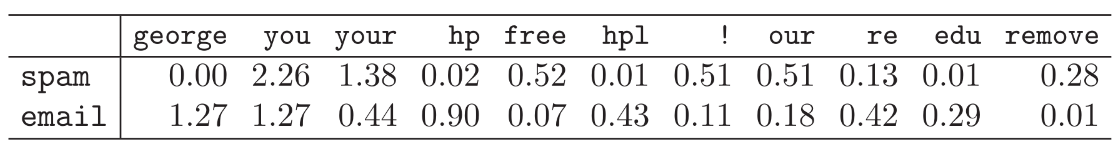
\includegraphics[scale=0.4]{images/table_1.png}\\
                Figura \thefigcount. Tabla donde se muestran las probabilidades de que cierta palabra aparezca en un correo del tipo \texttt{spam} y \texttt{email}.
                \stepcounter{figcount}
            \end{center}
        \end{minipage}

        Nuestro método de aprendizaje decide cuáles de características usar y como: Por ejemplo puede usar una regla como la siguiente:

        \begin{lstlisting}
if george < 0.6 & you > 1.5 then spam, else email. 
        \end{lstlisting}

        o también:

        \begin{lstlisting}
if 0.2*you - 0.3*george > 0 then spam, else email.
        \end{lstlisting}

        En este problema no todos los errores son iguales, queremos evitar filtrar email que realmente corresponda a \texttt{email}. Una forma de atacar este problema se discute más adelante.
    \end{sol}

    \begin{obs}
        No existe un lenguaje de programación usado en este texto a menos que se indique lo contrario. Si no parece que es algún lenguaje conocido, como el caso del ejercicio anterior, asumiremos que este es pseudocódigo.
    \end{obs}

    \begin{excer}[\textbf{Reconocimiento de Números en Manuscrita}]
        Se tienen miles de cartas escritas a mano con códigos postales en las mismas. Cada carta es escaneada y almacenada. De cada una de las cartas se extrae el área que contiene el código postal y se almacena. El objetivo es determinar el número que está escrito en el código postal.
    \end{excer}

    \begin{sol}
        Lo que se hace es primero, separar cada uno de los números en la imagen para después, colocar ese número en un grid de $16\times 16$ bits en escala de grises con cada uno de éstos variando de intensidad desde 0 hasta 255. Se pretende con esto determinar cada uno de los números en cada una de las imágenes.

        \begin{minipage}{\textwidth}
            \begin{center}
                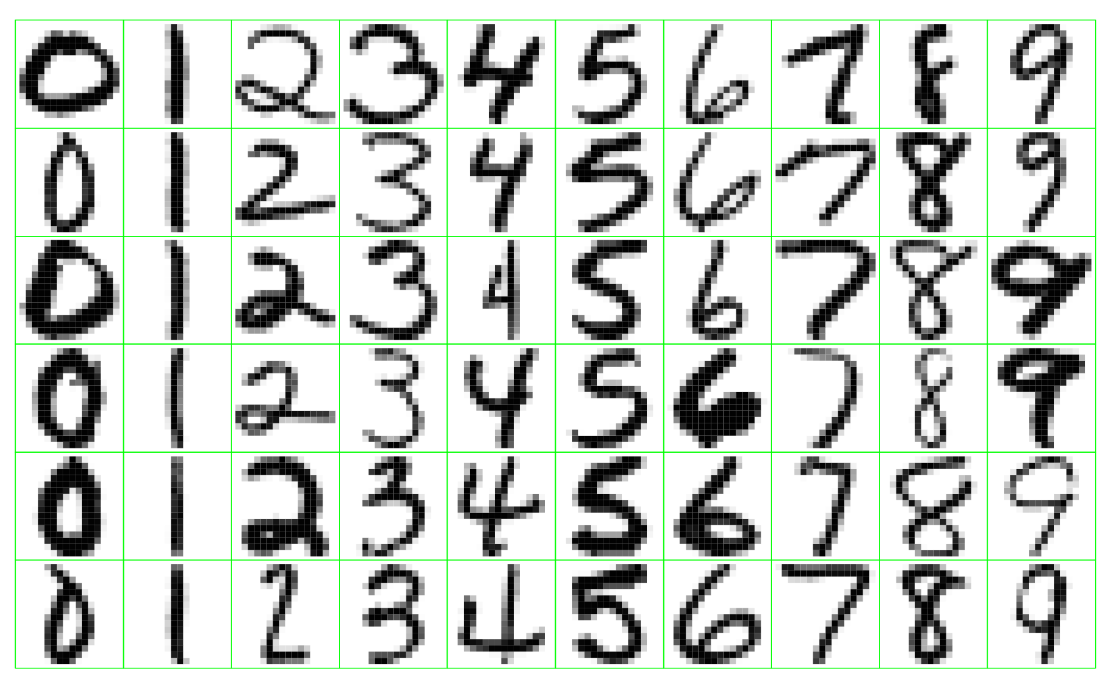
\includegraphics[scale=0.3]{images/image_1.png}\\
                Figura \thefigcount. Diversos números sacados de cartas en códigos postales.
                \stepcounter{figcount}
            \end{center}
        \end{minipage}

        Este es un problema de clasificación cuyo error debe mantenerse bajo para poder dar un resultado lo mejor posible.
    \end{sol}

    Otro problema inteeresante es el de \textit{regresión}, en el que básicamente se da un input de información varia y se requiere dar un output de cierto parámetro que puede o no ser deducido a partir de esos valores introducidos inicialmente.

    %TODO: Poner un problema de aprendizaje no supervisado

    Aplicar técnicas de Machine Learning para escarbar en una gran cantidad de información puede ayudar a descubrir patrones donde no es claro que éstos existan, esto es llamado \textbf{data mining}.

    Podemos aplicar las técnicas del Machine Learning en tres áreas:

    \begin{itemize}
        \item Supervisado o no supervisado (entran como subcategorías semisupervisado y aprendizaje con refuerzo).
        \item Online and Batch Learning.
        \item Si trabajan comparando nueva información con puntos de información ya existentes o si a partir de la información pueden obtener predicciones, como haría un científico.
    \end{itemize}

    Los algoritmos de aprendizaje supervisado más importantes son los siguientes:
    \begin{itemize}
        \item $k$-nearest neighbors.
        \item Linear Regresssion.
        \item Logistic Regression.
        \item Support Vector Machines (SVMs).
        \item Decision Trees and Random Forests.
        \item Neural Networks (algunas pueden ser no supervisadas o semisupervisadas).
    \end{itemize}

    En no supervisado:
    \begin{itemize}
        \item Clustering:
        \begin{itemize}
            \item $k$-means.
            \item DBSCAN.
            \item Hierarchical Cluster Analysis (HCA).
        \end{itemize}
        \item Anomaly detection and novelty detection:
        \begin{itemize}
            \item One-class SVM.
            \item Isolation Forest.
        \end{itemize}
        \item Visualization and dimensionality reduction:
        \begin{itemize}
            \item Principal Component Analysis
            \item Kernel PCA
            \item Locality Linear Embedding
            \item $t$-distributed stochastic neighbor embedding.
        \end{itemize}
        \item Association rule learning:
        \begin{itemize}
            \item A priori.
            \item Eclat.
        \end{itemize}
    \end{itemize}

    La gran mayoría de algoritmos de aprendizaje semisupervisado son mezclas de algorimos supervisados y no supervisados.

    El aprendizaje reforzado es muy diferente. Hay un \textit{agente} que recibe \textit{rewards} o \textit{penalties} en función de la acción que haga. Una política define que cosas debe elegir el \textit{agent} y cuales no, dada una situación.

    \chapter{Vista Panorámica del Aprendizaje Supervisado}

    \section{Introducción}

    El objetivo es que dada entrada de información demos una salida de la misma que podemos medir (ya que en aprendizaje supervisado eso es lo que se hace). Pueden ser muchas entradas de información de diferentes tipos y varias salidas igualmente de diferentes tipos.

    \begin{mydef}[\textbf{Terminología Machine Learning}]
        Los \textit{inputs} son a menudo llamados \textbf{predictors} o \textbf{independent variables} (\textbf{variables independientes} en español), los \textit{outputs} son llamados \textbf{responeses} o \textbf{variables dependientes} (\textbf{respuestas} en español). 
    \end{mydef}

    Se adoptará mucha terminología matemática vista en cursos de álgebra lineal y temas un poco más avanzados, por lo que no se ahondara mucho en ello. Sin embargo, es relevante mencionar el tipo de información con el que puede que estemos trabajando a menudo:

    %TODO: Poner tipos de input y output

    \section{Mínimos Cuadrados y Vecinos Cercanos}

    \begin{mydef}
        Si $\vec{x}$ es un vector $n$-dimensional, entenderemos que $\vec{x}$ es una matriz columna y así, $\vec{x}^T$ denotará a la transpuesta de esta matriz.
    \end{mydef}

    El modelo más simple de predicción es el modelo líneal. Si $\vec{x}=(x_1,x_2,...,x_n)$ es una entrada, entonces la salida del modelo líneal es el vector:
    \begin{equation}
        \vec{y}=\hat{\beta_0}+\sum_{ i=1}^n x_i\hat{\beta_j}
    \end{equation}
    donde $\hat{\beta_j}$ son vectores $m$-dimensionales para todo $j\in\natint{0,n}$. En particular, el vector $\hat{\beta_0}$ es llamado el \textbf{bias} en Machine Learning. Una forma más sencilla de representar lo anterior es haciendo $\vec{x'}=(1,x_1,...,x_n)$ y tomar:
    \begin{equation}
        \vec{y}=\vec{x'}^T\hat{\beta}
    \end{equation}
    donde $\hat{\beta}=(\hat{\beta_0},...,\hat{\beta_0})$. Notemos que en este caso las coordenadas $x_1,...,x_n$ del vector $\vec{x}$ son escalares y las de $\hat{\beta}$ pueden ser incluso vectores, con lo que $\hat{\beta}$ en general será una matriz. La salida tendrá la misma dimensión que las coordenadas de las entradas de $\hat{\beta}$.

    Podemos construir así la función:
    \begin{equation}
        f(\vec{x})=\vec{x'}^T\hat{\beta}
    \end{equation}
    esta es una función de un espacio $n$-dimensional en uno $m$-dimensional.

    Vista como función:
    \begin{equation}
        f(\vec{x})=\vec{x}^T\beta
    \end{equation}
    donde $\beta$ es una matriz $m\times n$ y es tal que $\nabla f(\vec{x})=\beta$, es decir lo clásico que uno hace en un curso de Cálculo III para determinar derivadas de transformaciones lineales.

    Nuestro objetivo es que este modelo lineal se acomple a nuestra información. Hay muchas formas de hacerlo pero la más sencilla es por \textbf{mínimos cuadrados}. En tal aproximación lo que uno hace es tomar los coeficientes de $\beta$ para minimizar el residuo de la suma de cuadrados:
    \begin{equation}
        \textup{RSS}(\beta)=\sum_{i=1}^k(y_i-\vec{x_i}^T\beta)^2
    \end{equation}
    la cosa anterior es un escalar (el cuadrado es el producto interno del vector resultante consigo mismo) y asumimos que tenemos un dataset de $k$-vectores. De forma más simplificada podemos escribir:
    \begin{equation}
        \textup{RSS}(\beta)=(\vec{y}-X^T\beta)^T(\vec{y}-X^T\beta)
    \end{equation}
    donde $\vec{y}=(y_1,...,y_n)$ y $X=(\vec{x_1},...,\vec{x_k})$. Notemos que $X^T\beta$ define la dimensión de las coordenadas del vector $\vec{y}$.

    Se tiene que $X$ tiene a cada columna como un vector de entrada $\vec{x_i}$ y la salida está dada por $y_i$, esto en el conjunto de entrenamiento.

    Esto es la cosa más simple del mundo de hacer en programación. Considere el siguiente ejemplo:

    \begin{exa}
        Se tiene un documento .csv donde se encuestó a personas de ciudades con cierto \textit{GDP per cápita (USD)} sobre su satisfacción de vida. Dada cierto GDP per cápita, determine la satisfacción de vida de la persona.
    \end{exa}

    \begin{sol}
        Este claramente es un modelo de regresión. Observemos primero un plot de la información para inferir si es que hay algo que podamos determinar de ella:

        \begin{minipage}{\textwidth}
            \begin{center}
                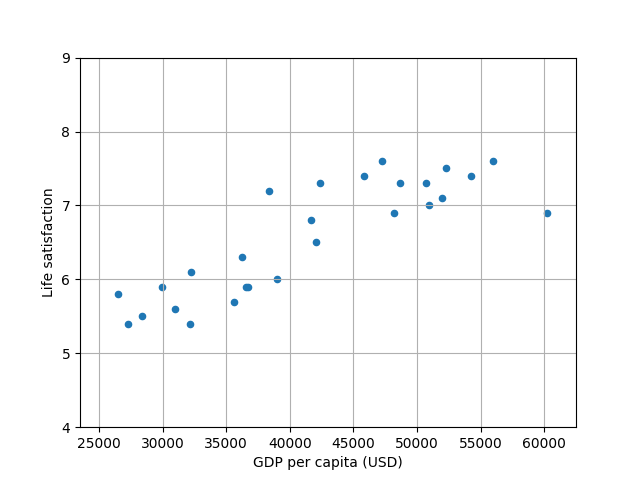
\includegraphics[scale=0.7]{images/plot_1.png}\\
                Figura \thefigcount. Caption.
                \stepcounter{figcount}
            \end{center}
        \end{minipage}

        rápidamente uno puede ver que tal vez haya alguna relación lineal, por lo que se implementa el siguiente código en Python para realizar un modelo de regresión lineal:
        
        \lstinputlisting[language=python,caption=Ejemplo Regresión Lineal]{code/introduccion.py}

        El modelo lo que hizo fue generar la siguiente línea recta roja:

        \begin{minipage}{\textwidth}
            \begin{center}
                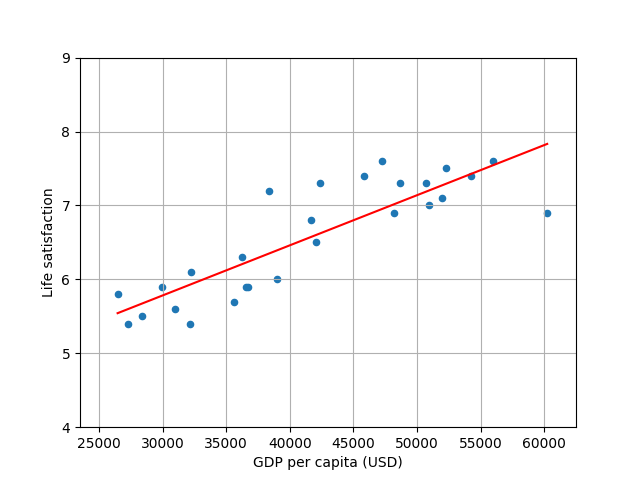
\includegraphics[scale=0.7]{images/plot_2.png}\\
                Figura \thefigcount. Caption.
                \stepcounter{figcount}
            \end{center}
        \end{minipage}

        Con este mismo ejemplo podemos implementar otro modelo, por ejemplo el de $k$-nearest neighbors con $k=3$.

        \lstinputlisting[language=python,caption=Ejemplo $k$-vecinos]{code/knn_1.py}

        En este caso, la gráfica queda de la siguiente manera:

        \begin{minipage}{\textwidth}
            \begin{center}
                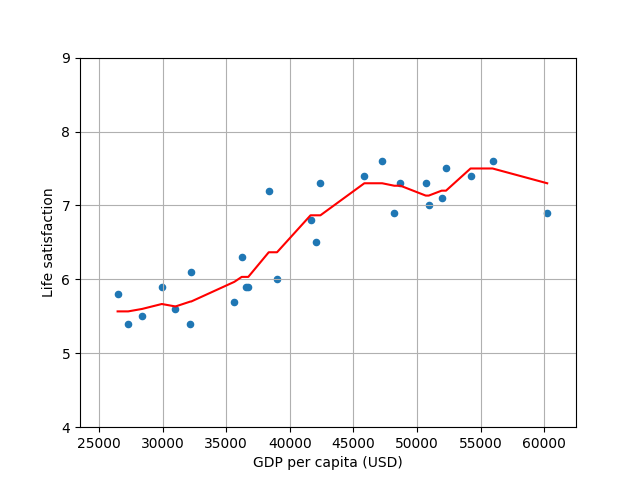
\includegraphics[scale=0.7]{images/plot_3.png}\\
                Figura \thefigcount. Caption.
                \stepcounter{figcount}
            \end{center}
        \end{minipage}

        El algoritmo de regresión lo que hace (de forma descriptiva) es encontrar los $k$ vecinos más cercanos de un punto y hace el promedio de los valores.

    \end{sol}
    
    En síntesis, se siguen los 4 siguientes pasos:

    \begin{itemize}
        \item Estudiar la información.
        \item Limpiar la información.
        \item Preparar la información.
        \item Seleccionar un modelo.
        \item Entrenar el modelo con la información de entrenamiento.
        \item Aplicar el modelo para hacer predicciones.
    \end{itemize}

\end{document}

\begin{minipage}{\textwidth}
    \begin{center}
        %\includegraphics[scale=0.5]{direccion_imagen}\\
        Figura \thefigcount. Caption.
        \stepcounter{figcount}
    \end{center}
\end{minipage}